%%%%%%%%%%%%%%%%%%%%%%%%%%%%%%%%%%%%%%%%%%%%%%%%%%%%%%%%%%%%%%%%%%%%%%%%%%%%%%%
% Evaluating GenAI-Based Information Extraction and Classification
% NLP Lab SoSe 2026 — Technical University of Munich
% Team 38: Amine Smaoui, Ismail Ege Oguz, Robert Pham
% Industry partner: Carl Zeiss AG (Dr. Georg Dietrich, Dr. Maximilian Wich)
%
% BUILD:  latexmk -pdf main.tex (requires Perl), or pdflatex -> bibtex -> pdflatex x2
% STYLE:  layout lives in tumpaper.sty; content lives in sections/*.tex
% REFS:   add entries to references.bib, cite with \citep{key} / \citet{key}
%%%%%%%%%%%%%%%%%%%%%%%%%%%%%%%%%%%%%%%%%%%%%%%%%%%%%%%%%%%%%%%%%%%%%%%%%%%%%%%

% Two-column, 10 pt: the conference-paper format the 8-page limit assumes.
% For a single-column version (e.g. a thesis chapter), remove `twocolumn` here
% and switch the starred floats in the section files back to unstarred.
\documentclass[
    fontsize=10pt,
    a4paper,
    twoside=false,
    twocolumn,
    numbers=noendperiod
]{scrartcl}

\usepackage{tumpaper}  % all layout, colors, packages — see tumpaper.sty

% Running head (appears in the page header from page 2 onward; page 1 carries
% the title block instead, so the header is suppressed there).
\setrunningtitle{Evaluation and Human-in-the-Loop Annotation with GenAI}
\setrunningauthor{Amine Smaoui, Ismail Ege Oguz, Robert Pham}

\begin{document}

%%%%%%%%%%%%%%%%%%%%%%%%%%%%%%%%%%%%%%%%%%%%%%%%%%%%%%%%%%%%%%%%%%%%%%%%%%%%%%%
% TITLE BLOCK — spans both columns at the top of page 1
%%%%%%%%%%%%%%%%%%%%%%%%%%%%%%%%%%%%%%%%%%%%%%%%%%%%%%%%%%%%%%%%%%%%%%%%%%%%%%%
\twocolumn[\begin{tumtitleblock}

% The logo sits flush with the right text margin, on the same baseline block as
% the rule underneath it, so the two right edges line up exactly.
\vspace*{-6mm}
\noindent\hfill{
\includegraphics[height=11mm]{figures/tum_logo.pdf}}

\vspace{2.5mm}
\noindent{\color{TUMBlue}\rule{\textwidth}{1pt}}

\vspace{3mm}
\noindent{\raggedright\sffamily
{\fontsize{18pt}{21pt}\selectfont\bfseries\color{TUMBlue}
Evaluation and Human-in-the-Loop Annotation\\Using GenAI Approaches\par}

\vspace{2mm}
{\fontsize{12pt}{14pt}\selectfont\color{TUMDarkBlue}
A Reproducible Framework for Classification, Document-Scale Extraction,
and Reviewed Gold Data\par}
}

\vspace{2.5mm}
\noindent{\color{TUMBlue}\rule{\textwidth}{0.5pt}}

\vspace{4mm}
\noindent{\raggedright\sffamily
{\bfseries Amine Smaoui \;\textperiodcentered\; Ismail Ege Oguz \;\textperiodcentered\; Robert Pham\par}
\vspace{1.2mm}
{\small School of Computation, Information and Technology,
Technical University of Munich\par}
\vspace{0.6mm}
{\small NLP Lab, Summer Semester 2026. Supervised by Dr.\ Georg Dietrich and
Dr.\ Maximilian Wich, Carl Zeiss AG.\par}
}

\vspace{5mm}
% ============================================================================
% ABSTRACT + KEYWORDS  —  owner: TBD  —  ~220 words
% Formula: context -> gap -> what we did -> what we found -> what it means.
% ============================================================================
\begin{abstract}
\noindent
Large language models (LLMs) make information extraction and ticket
classification available without task-specific training, but useful deployment
still requires evidence on the target data and an efficient way to create that
evidence. We present a reproducible evaluation framework and a configurable
human-in-the-loop annotation application. The framework preserves raw model
responses, validates spans and labels, and reports strict and reviewer-oriented
metrics. The application suggests a schema-derived prompt, pre-annotates text,
PDF, or CSV input, supports optional department routing through either an
editable LLM prompt or a local embedding vote over reviewed tickets, records
every reviewer correction, and exports traceable gold JSON. On a fresh
held-out sample of 20
SciREX papers, four-type scientific mention extraction reached $57.38\%$
strict $F_1$ (document-bootstrap 95\% interval $53.56$--$60.73$), $67.36\%$
boundary-tolerant $F_1$, and $70.30\%$ same-label overlap $F_1$. A completed
100-paper full-window operational run processed 8{,}373 sentences and 9{,}901
gold mentions with no failed document, achieving $54.09\%$ strict and
$66.22\%$ overlap $F_1$. Earlier baselines show $79.32\%$ strict $F_1$ for
single-type Few-NERD extraction and $72.6\%$ type accuracy but only $42.2\%$
queue accuracy on synthetic support tickets. The results show that exact span
quality, label semantics, and target-domain evaluation matter more than output
validity alone, and that LLM predictions should remain reviewer suggestions
rather than ground truth.
\end{abstract}

\noindent\textbf{Keywords:} information extraction; text classification;
large language models; long documents; evaluation framework;
human-in-the-loop annotation; reproducibility
\vspace{4mm}

\vspace{3mm}

\end{tumtitleblock}]

% No running header on page 1: the title block already identifies the paper.
\thispagestyle{plain}

% Set \showtoc to 1 while drafting to get a table of contents; keep it at 0 for
% the 8-page submission version.
\newcommand{\showtoc}{0}
\ifnum\showtoc=1 \tableofcontents\clearpage \fi

%%%%%%%%%%%%%%%%%%%%%%%%%%%%%%%%%%%%%%%%%%%%%%%%%%%%%%%%%%%%%%%%%%%%%%%%%%%%%%%
% BODY
%%%%%%%%%%%%%%%%%%%%%%%%%%%%%%%%%%%%%%%%%%%%%%%%%%%%%%%%%%%%%%%%%%%%%%%%%%%%%%%
% ============================================================================
% 1 INTRODUCTION  —  target: ~0.9 page
% ============================================================================
\section{Introduction}
\label{sec:introduction}

Information extraction (IE) and text classification turn unstructured text
into structured, usable data. A service engineer repairs a machine and records
the customer request, the observed failure, and the corrective action. Across
thousands of reports, these records contain information required for quality
analysis in a form that conventional dashboards cannot directly process. IE
extracts the relevant facts, whereas classification assigns each document to a
category \citep{xu2024generative}.

\begin{figure*}[!t]
\centering
\resizebox{\textwidth}{!}{%
\begin{tikzpicture}[node distance=4mm]
% ---- Row 1: classical supervised ML -------------------------------------
\node[tumdata] (c1) {Large ticket set};
\node[tumbox, right=7mm of c1] (c2) {Labeling by\\domain expert\\\scriptsize slow and expensive};
\node[tumdata, right=7mm of c2] (c3) {Train / test split};
\node[tumbox, right=7mm of c3] (c4) {Train and tune\\\scriptsize by an ML expert};
\node[tumdata, right=7mm of c4] (c5) {Inference};
\foreach \a/\b in {c1/c2, c2/c3, c3/c4, c4/c5} \draw[tumarrow] (\a) -- (\b);
\node[tumlabel, left=5mm of c1, align=right, anchor=east] {\textbf{(a) Classical ML}};

% ---- Row 2: LLM only ----------------------------------------------------
\node[tumdata, below=9mm of c1] (l1) {Large ticket set};
\node[tumbox, right=7mm of l1] (l2) {LLM};
\node[tumdata, right=7mm of l2] (l3) {Inference};
\foreach \a/\b in {l1/l2, l2/l3} \draw[tumarrow] (\a) -- (\b);
\node[tumlabel, left=5mm of l1, align=right, anchor=east] {\textbf{(b) LLM only}};
\node[tumlabel, right=7mm of l3, text=TUMOrange, align=left, anchor=west]
  {\;$\leftarrow$ no step here measures how well it works};

% ---- Row 3: LLM with evaluation (what we built) -------------------------
\node[tumdata, below=9mm of l1] (e1) {Large ticket set};
\node[tumbox2, right=7mm of e1] (e2) {\textbf{Step 1}\\LLM pre-annotation\\\scriptsize spans, labels, offsets};
\node[tumbox2, right=7mm of e2] (e3) {\textbf{Step 2}\\Expert validation\\\scriptsize confirm $\cdot$ correct $\cdot$ delete};
\node[tumdata, right=7mm of e3] (e4) {Gold test set};
\node[tumbox, right=7mm of e4] (e5) {Evaluation\\\scriptsize P / R / F$_1$};
\node[tumdata, right=7mm of e5] (e6) {Inference};
\foreach \a/\b in {e1/e2, e2/e3, e3/e4, e4/e5, e5/e6} \draw[tumarrow] (\a) -- (\b);
\node[tumlabel, left=5mm of e1, align=right, anchor=east] {\textbf{(c) LLM with evaluation}};

\begin{scope}[on background layer]
\node[draw=TUMOrange!50, dashed, rounded corners=3pt, inner sep=6pt, fit=(e2)(e3)] (tool) {};
\node[draw=TUMBlue!40, dashed, rounded corners=3pt, inner sep=6pt, fit=(e5)] (fw) {};
\end{scope}
\node[tumlabel, below=1mm of tool.south, anchor=north, text=TUMOrange] {annotation tool};
\node[tumlabel, below=1mm of fw.south, anchor=north, text=TUMBlue] {evaluation framework};
\end{tikzpicture}%
}
\caption{Three annotation workflows. (a)~The supervised pipeline requires
expert labeling before model development. (b)~Direct LLM inference omits an
independently labeled evaluation set. (c)~The implemented workflow combines
LLM pre-annotation with expert validation and gold-set evaluation. Dashed
boxes denote the two artifacts developed in this project.}
\label{fig:workflows}
\end{figure*}

Until recently, this process required substantial initial investment,
workflow~(a) in \Cref{fig:workflows}: domain experts labeled thousands of
examples, machine-learning specialists trained and tuned a model, and label-set
changes could require additional annotation and training. Instruction-tuned
large language models (LLMs) reduce this initial effort because a task can be
specified through label descriptions and examples in a prompt, workflow~(b).

The principal limitation is the loss of independent evaluation data. The
labels created for supervised learning also served as a test set against which
predictions could be measured. Organizations may therefore lack annotations
for their target domain and cannot reliably evaluate deployed models. Vendor
benchmarks may differ substantially from service reports, while informal spot
checks cannot establish deployment quality. LLM annotation quality varies
across tasks and datasets and must therefore be measured against human labels
rather than assumed
\citep{pangakis2023validation, reiss2023testing}.

Workflow~(c) is implemented in this study. An LLM pre-annotates, a domain expert
validates, and the result is a small gold set to measure against. We built both
halves: an evaluation framework for classification and span extraction, and a
configurable annotation product that turns model output into reviewed data.
The initial Few-NERD and support-ticket experiments test method and output
choices on short inputs. The later SciREX study addresses the harder operational
case: coherent scientific text ranging from one sentence to more than 200,
processed completely with durable checkpoints and evaluated against released
span annotations \citep{jain2020scirex}. This progression matters because
sentence-local predictions that work on isolated inputs must still be shown to
cover every sentence in a full document reliably and economically.

\paragraph{Contributions.}
Our contributions are threefold. First, we provide a task-separated,
configuration-driven evaluation framework that stores raw responses and scores
them independently of inference. Second, we construct a reproducible
1{,}000-window SciREX benchmark from 438 source papers while preserving source
order, document identity, split membership, and exact character offsets; the
completed study stages include a development prompt comparison, a fresh
20-paper held-out confirmation, and a 100-paper full-window operational run.
Third, we deliver a Dockerized annotation application with schema-derived but
editable prompts, arbitrary labels, text/PDF/CSV input, optional reviewer-
approved LLM or local-embedding ticket routing, confidence-ranked review, and
auditable JSON export.
Together, these artifacts define a reproducible process from unlabeled
organizational text to an evaluation set with inspectable provenance.
      % motivation, the three workflows, contributions
% ============================================================================
% 2 STATE OF THE ART AND THEMATIC ANALYSIS  —  the literature review.
% Organized BY THEME, not by paper. Each theme ends with the design decision
% it produced. Kept tight: the 8-page limit includes the bibliography.
% ============================================================================
\section{State of the Art and Thematic Analysis}
\label{sec:related}

We read work published between 2018 and 2025, mostly peer-reviewed and from the
main NLP and machine-learning venues (ACL, EMNLP, NAACL, EACL, COLING, ICLR,
NeurIPS), from reviewed journals (\emph{PNAS}, \emph{Computational
Linguistics}, \emph{Frontiers of Computer Science}, \emph{JMIR Medical
Informatics}), or from CHI and WWW for the human-in-the-loop side. Seven sources
are arXiv preprints, kept only where the work is widely cited and from an
identifiable group, and marked as preprints rather than treated as reviewed.
Sources had to speak to one of four questions: how well prompted models extract
and classify, how their output should be shaped, how a reviewer should be
pointed at the doubtful cases, and how any of it can be checked without gold
data. Eight themes follow.

\paragraph{From supervised pipelines to prompted generalists.}
\citet{xu2024generative} survey generative IE. Generative formulations can
accommodate dynamically specified labels through natural-language descriptions,
avoiding a fixed classifier output layer. Specialized instruction-tuned systems
such as InstructUIE \citep{wang2023instructuie} and targeted-distillation systems
such as UniversalNER \citep{zhou2024universalner} demonstrate that
task-specialized smaller models can outperform general-purpose prompted LLMs on
IE benchmarks. GLiNER \citep{zaratiana2024gliner} makes a related point from the
encoder side: a bidirectional encoder matches LLM prompting at a fraction of
the inference cost.
\textbf{In our project,} fine-tuning was out of scope: we had access to one
hosted model and no permission to train on company data. So we compare only
methods that need no training step.

\paragraph{How far prompting alone gets on extraction.}
\citet{han2023solved} ask whether IE is solved by ChatGPT and answer no:
performance holds on tasks rewarding reasoning and drops on sequence labeling,
where boundaries count. \citet{xie2023empirical} show that decomposing NER into
simpler label-specific questions can substantially improve zero-shot
performance. \citet{sivarajkumar2024empirical} compare six prompt types across five
clinical tasks and find no overall winner, so prompt design must be tested per
task. GPT-NER \citep{wang2023gptner} adds a self-verification step asking
whether an extracted span really belongs to the target type.
\textbf{In our project,} two of these claims are testable, so we test both
(H1, H3).

\paragraph{Document-level scientific extraction.}
SciREX was introduced specifically because sentence- and paragraph-level IE
misses information distributed across scientific documents
\citep{jain2020scirex}. It annotates mentions of Method, Task, Metric and
Dataset as well as coreference, salience and document-level relations. Our
study uses its mention spans as externally supplied reference annotations; it
does not attempt the original paper's coreference or $n$-ary relation tasks.
This distinction prevents a misleading direct comparison between our
pre-annotation score and the SciREX end-to-end relation baseline.

\paragraph{Classification without training data, and label-set size.}
\citet{yin2019benchmarking} turn classification into natural language inference
with each label as a hypothesis, which works for any label set at inference
time but reacts strongly to wording. The embedding alternative encodes text and
label descriptions and selects the nearest representation
\citep{reimers2019sentence}; it is computationally inexpensive, local, and
requires no LLM call, and SetFit \citep{tunstall2022efficient}
shows how much it gains from eight labeled examples per class. MTEB
\citep{muennighoff2023mteb} is the usual way to choose an encoder. The harder
problem is scale: \citet{bhambhoria2023simple} show that flat zero-shot
classification degrades on layered label sets and that splitting the
decision into entailment steps recovers much of the loss, TELEClass
\citep{zhang2025teleclass} adds class-indicative terms to the label set,
and HierPrompt \citep{zhang2025hierprompt} builds hierarchy-aware prototypes.
All three assume that putting hundreds of labels in one prompt does not work.
\textbf{In our project,} the label sets have 4, 10 and several hundred values,
so we can watch this drop happen inside one dataset (H2).

\paragraph{Output format is not a free choice.}
\citet{tam2024speak} show format restrictions measurably hurt reasoning, and
tighter constraints hurt more, though structured formats \emph{help}
classification, where the task is choosing rather than reasoning. Span
extraction additionally needs offsets consistent with the emitted text, which
no JSON schema checks.
\textbf{In our project,} each extraction method exists twice, structured and
free-form, with accuracy and structural validity measured separately.

\paragraph{Whether an agentic step helps.}
\citet{huang2024selfcorrect} study intrinsic self-correction and find
performance usually does not improve and can get worse, because the model has
no independent signal about which parts were wrong. Work on LLMs as judges
documents position, verbosity and self-preference biases pointing the same way
\citep{zheng2023judging}.
\textbf{In our project,} we treated ``agentic helps'' as a hypothesis to test
rather than assume, and built two agentic variants for it (H3).

\paragraph{LLMs as annotators, and why validation is not optional.}
\citet{gilardi2023chatgpt} report ChatGPT beating crowd workers on several
annotation tasks at a fraction of the cost. The careful work came soon after.
\citet{ziems2024transform} test 13 models on 25 benchmarks and find fair
agreement with human coders but no win over fine-tuned models,
\citet{reiss2023testing} shows non-determinism alone can push consistency below
accepted reliability thresholds, and \citet{pangakis2023validation} replicate
27 tasks across 11 datasets and conclude every task needs its own check against
human labels. \citet{baumann2025hacking} quantify the downstream risk: across
13 million annotations feeding 1.4 million regressions, ordinary choices of
model and prompt wording sufficed to flip statistical conclusions. See
\citet{tan2024annotation} for a survey.
\textbf{In our project,} this theme is the reason the project exists. It also
fixes one rule for the tool: every human decision gets stored, because the
record of disagreement is the evidence.

\paragraph{Prioritizing uncertain cases for review.}
A reviewer facing forty plausible suggestions stops reading them properly, so
the tool must rank them. \citet{geng2024survey} survey confidence estimation
and split it into white-box methods reading internal signals such as token
probabilities and black-box methods treating the model as opaque;
\citet{kadavath2022know} show large models carry usable self-knowledge in their
probabilities. The black-box route is sampling: \citet{wang2023selfconsistency}
aggregate several sampled generations and \citet{kuhn2023semantic} refine this
further by grouping samples that mean the same thing before counting them.
\citet{xiong2024express} compare the families and report two findings we relied
on: models are overconfident when stating confidence in words, and white-box
methods beat black-box ones only narrowly. For annotation specifically,
\citet{wang2024collaborative} study how to make human verification effective
rather than mechanical.
\textbf{In our project,} the annotation tool supports multiple confidence
signals for prioritizing review; a systematic comparison of their calibration,
review utility, and additional cost remains future work.

\paragraph{Keeping the human in the loop.}
INCEpTION \citep{klie2018inception} already paired automatic suggestions with
human curation before LLMs; MEGAnno+ \citep{kim2024meganno} splits the work as
we do, with LLM agents proposing and people verifying. For annotation quality
the standard vocabulary is \citet{artstein2008intercoder}.
\textbf{In our project,} we took that two-step design, adapted it to span-level
extraction with character offsets, and logged every accept, relabel and
delete.

\paragraph{The integration considered here.}
Existing work studies individual components of this process, but we did not
find a single task-separated workflow combining reproducible LLM inference,
independently scored extraction and classification, reviewer correction,
provenance, and reusable gold-data export for the target setting considered
here. This project implements and evaluates that specific integration.
      % state of the art + thematic literature analysis
% ============================================================================
% 3 PROBLEM STATEMENT AND RESEARCH QUESTIONS
% ============================================================================
\section{Problem Statement and Research Questions}
\label{sec:problem}

An organization can obtain plausible extraction and classification output from
a general LLM without training a task-specific model. Plausibility is not an
accuracy measure, however, and the organization usually lacks reference labels
for exactly the documents it wants to process. It must therefore solve two
linked engineering problems: evaluate a proposed method on representative
data, and create trustworthy annotations without making experts label every
document from scratch. Long documents add operational concerns---call volume,
partial failures, offset reconstruction and resumability---that short benchmark
sentences conceal.

We address the following questions:

\begin{description}[leftmargin=1.7cm, style=nextline, font=\bfseries, itemsep=1pt]
    \item[RQ1] How accurately and reliably does a training-free LLM reproduce
        reference labels for ticket classification and span extraction, under
        strict structural and semantic validation?
    \item[RQ2] How well does schema-guided pre-annotation localize Method,
        Task, Metric and Dataset mentions in coherent SciREX text using
        sentence-local predictions, and how does performance change from short
        to very long document windows?
    \item[RQ3] Can one reusable human-in-the-loop product turn model
        predictions into auditable reviewed data across scientific extraction
        and internal-ticket use cases?
\end{description}

The study is intentionally not a model leaderboard. A single hosted deployment
is fixed so that changes in data, prompt and pipeline remain visible. We use
strict span $F_1$ as the primary extraction measure, because a gold export must
reproduce exact offsets, and predeclare boundary-tolerant and overlap metrics as
secondary measures of whether a suggestion still directs a reviewer to the
useful phrase. For document-scale evaluation, source paper rather than window is
the statistical unit because several windows may originate from one paper.

Three expectations guide the analysis. First, syntactically valid JSON will not
guarantee correct labels or boundaries. Second, schema definitions and explicit
negative guidance will materially affect extraction quality. Third, a complete
document-scale run should be technically possible through sentence-level
checkpointing, but accuracy need not improve with longer windows because calls
remain sentence-local. These are evaluated only where retained artifacts support
the comparison; unexecuted configurations are not presented as results.
           % problem statement, research questions, hypotheses
% ============================================================================
% 4 METHODOLOGY
% ============================================================================
\section{Methodology}
\label{sec:methodology}

\paragraph{Experimental control and provenance.}
All reported LLM runs use the configured \code{hosted:gpt-5.4} deployment at
temperature $0$. Each prediction record stores the example and document IDs,
model and method, raw and parsed output, prompt and manifest hashes, token
usage, elapsed time and validation state. Evaluation is a separate deterministic
step, so alternative matching policies can be applied without another API call.
We report only conditions backed by retained prediction and score artifacts.

\paragraph{Short-input baselines.}
Ticket classification predicts one \labelname{type}, one \labelname{queue} and
a set of \labelname{tags}. A zero-shot call selects from allowed values and
quotes evidence; an agentic two-step method first extracts evidence and then
maps it to labels. Both completed the same 1{,}000-ticket slice. Few-shot
classification is implemented but only smoke-tested on one row and is excluded
from comparison. Embedding-based retrieval of reviewed tickets is also
implemented as an optional dynamic few-shot method, but no leakage-safe
reference/development/test split was available for the reported synthetic-ticket
experiment; consequently, it is not included in the reported comparison. For
interactive use, the annotation application additionally implements a pure
nearest-neighbor router: it embeds a ticket locally and applies a
similarity-weighted vote over reviewed reference tickets, without making a
routing LLM call. This route is likewise excluded from the reported accuracy
results because it has not yet been tested on an independent target-domain
split. For Few-NERD, the two directly comparable 1{,}000-sentence
conditions are few-shot structured JSON and few-shot free-form output, each
using three training examples and explicit inclusive token indices. The
zero-shot extraction artifacts contain 100 examples and are reported only as a
supplementary scale check, not as a full-slice comparison.

\paragraph{SciREX prompt selection and frozen evaluation.}
The application derives a deterministic prompt from the active label schema,
definitions and domain guidance; this suggestion costs no LLM call and remains
editable. On a fixed 20-paper development sample, we compared the previous
static few-shot prompt with this suggestion using the first ten app-detected
sentences per window. The selected prompt presents Method, Task, Metric and
Dataset to users; Dataset is mapped to SciREX's release label Material during
evaluation. After prompt selection, a fresh 20-paper official-test sample,
excluding test papers already inspected, was processed in full. A separate
100-paper training-split gate, balanced across four length buckets, tested full
coverage, throughput and failure recovery. No test result was used to revise
the reported prompt.

\paragraph{Document-scale execution.}
Windows are split into sentences only for API calls; all sentences are processed
when \code{max\_sentences=0}. Four workers handle independent documents. Before
each call and after each successful sentence, state is written atomically.
Repeating an identical command resumes at the next unfinished sentence, while
hash checks reject mixed manifests, models or prompts. The runner enforces call
and request-rate ceilings, retries transient failures, and records missing usage
and invalid responses. Provider prices were unavailable, so monetary cost is
not inferred from token counts.

\paragraph{Metrics.}
For extraction, strict one-to-one matching requires the same case-insensitive
label and exact half-open character span. Boundary-tolerant matching permits a
start within one token and an end within two; overlap matching accepts any
same-label character overlap. Strict is primary; the other two quantify useful
localization for human review. We report micro precision, recall and $F_1$,
macro-document $F_1$, per-label and length-bucket results. Uncertainty intervals
use 2{,}000 percentile-bootstrap samples clustered by source \code{doc\_id}.
Ticket single-label fields use accuracy and macro-$F_1$; multi-label tags use
micro-$F_1$. Invalid JSON, invalid labels, evidence validity, failures, token
usage and coverage are reported as operational measures.
       % how we address the questions
% ============================================================================
% 5 DATA
% ============================================================================
\section{Data}
\label{sec:data}

No confidential industrial ticket or service-report data is used. The public
datasets test mechanics and establish baselines; they do not substitute for an
evaluation on the deployment organization's own distribution.

\paragraph{Synthetic support tickets.}
The multilingual customer-support collection \citep{bueck2024tickets} contains
English and German synthetic emails with provided routing fields. Our processed
table has 24{,}743 rows; experiments use a fixed first slice of 1{,}000. The
label spaces contain 4 ticket types, 10 queues, and 1{,}129 observed tag strings.
The tags deliberately remain noisy, including case variants, misspellings and
comma-joined values. These are dataset-provided reference labels, not expert
annotations from the intended deployment, so results measure reproduction of
this synthetic labeling policy.

\paragraph{Few-NERD.}
Few-NERD \citep{ding2021fewnerd} contains 188{,}238 Wikipedia sentences with 8
coarse and 66 fine types. We use a deterministic 1{,}000-sentence location-only
slice from the intra test split for the directly comparable few-shot runs.
Token-level reference spans make it a useful regression test for prompt parsing
and offset reconstruction, although isolated Wikipedia sentences do not test
document-scale execution.

\paragraph{SciREX.}
SciREX \citep{jain2020scirex} provides complete tokenized scientific papers with
Method, Task, Metric and Dataset/Material mention spans, created through a
combination of automatic and human annotation. The release used here contains
438 documents, 120{,}432 sentences and 156{,}931 mention spans. Preprocessing
detokenizes each document deterministically, converts exclusive token offsets
to validated half-open character offsets, and preserves the original
train/development/test split.

From these papers we construct 1{,}000 contiguous same-document windows, 250 in
each bucket: short (1--10 sentences), medium (11--50), long (51--200), and very
long (at least 201). Sentence order is never randomized. Windows from a paper
may overlap by at most 50\%, so \code{doc\_id} must be retained for splitting
and uncertainty estimation. The full benchmark contains 109{,}138 gold mentions
and is available as linked example, sentence and entity CSV tables. The
completed 100-paper operational subset contains 25 unique training papers per
bucket, 8{,}373 sentences and 9{,}901 mentions. The fresh held-out confirmation
contains 20 different official-test papers, 1{,}633 sentences and 2{,}359
mentions. The configured 1{,}000-window run remains prepared but was not
completed and is therefore not reported as an empirical result.
              % datasets and their properties
% ============================================================================
% 6 ARCHITECTURE AND SOLUTION DESIGN
% ============================================================================
\section{Architecture and Solution Design}
\label{sec:architecture}

Two artifacts implement workflow~(c) of \Cref{fig:workflows}: an evaluation
framework for data with reference labels and an annotation product for creating
reviewed labels where none exist.

\subsection{Evaluation framework}

The Python repository is separated by task. Configuration and prompt files
describe a run; method classes expose a common prediction interface; runners
handle API calls, retries and validation; evaluators read stored predictions and
write aggregate, per-example, per-label and error artifacts. The SciREX adapter
adds deterministic detokenization, document-window construction and offset
assertions. A production batch runner adds atomic sentence checkpoints,
configuration hashes, bounded parallelism, rate and call ceilings, token
accounting and idempotent resume. This separation is important: inference is
expensive and stateful, whereas scoring should be computationally inexpensive,
inspectable, and repeatable.

For ticket classification, an optional dense-retrieval component indexes
reviewed reference tickets with a pretrained sentence encoder and supplies the
nearest valid examples to the LLM prompt. The index manifest stores source and
artifact hashes, encoder identity, dimensions and column mappings. Reference
and evaluation data remain separate, and query-time exclusion by ticket ID and
normalized text provides an additional leakage safeguard. This component is a
retrieval baseline, not LLM fine-tuning, and remains excluded from reported
results until it is evaluated on an independent internal split.

\subsection{Human-in-the-loop annotation product}

The Streamlit application accepts pasted text, TXT, PDF, or an interactively
mapped CSV row. A user selects or copies a YAML use-case template, edits labels
and the complete schema-derived prompt, chooses an OpenAI-compatible or local
Ollama model, and runs pre-annotation. Suggestions are highlighted in context
and listed with exact character offsets, provenance, status and confidence
(\Cref{fig:tool}). Reviewers can confirm, relabel, delete, adjust or add spans.
The export retains immutable model predictions alongside final
\code{gold\_entities}, prompt hashes, token usage and the full review history.

\begin{figure*}[!t]
\centering
{\setlength{\fboxsep}{0pt}\setlength{\fboxrule}{0.4pt}%
 \fcolorbox{TUMLightGray}{white}{%
 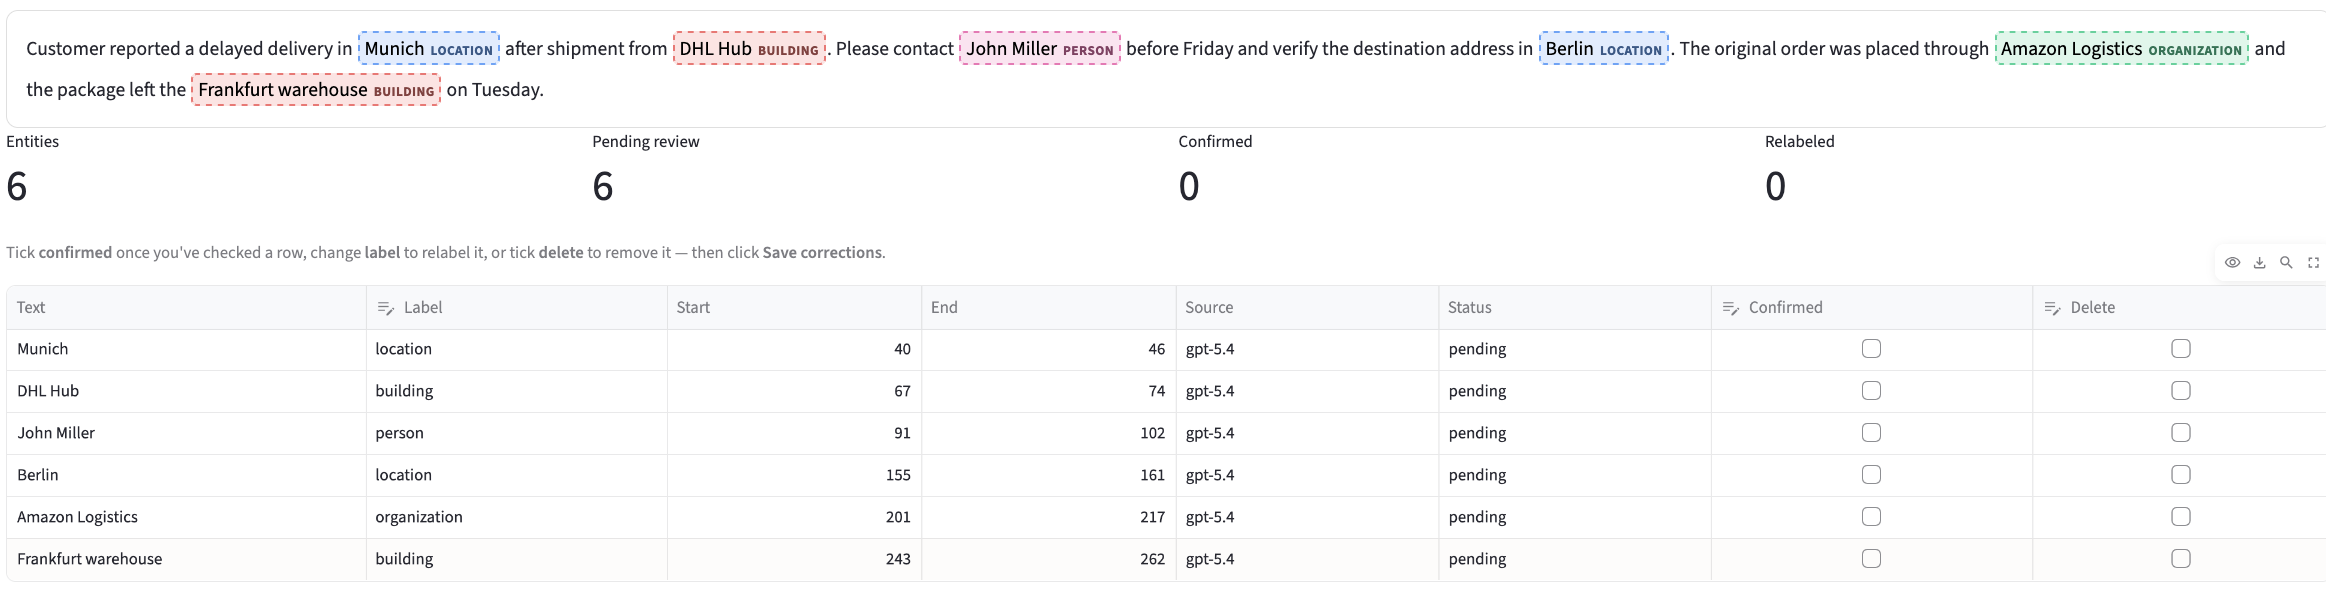
\includegraphics[width=\dimexpr\textwidth-0.8pt\relax]{figures/annotation_review.png}}}
\caption{Human review in the annotation product. Model spans are highlighted
in the source text and exposed as editable records; corrections and deletions
remain part of the audit trail rather than being overwritten.}
\label{fig:tool}
\end{figure*}

\paragraph{Reusable domain configuration.}
YAML templates currently cover general named entities, scientific IE and
internal support tickets. Each defines labels, descriptions, domain guidance
and optional routing destinations. The prompt suggestion is deterministic, so
it is reproducible and free, but the user can adapt it before inference. Custom
labels receive a generic starting definition instead of disabling the tool.

\paragraph{Optional classification before extraction.}
For tickets, the user selects either an LLM classifier or a local embedding
classifier. The LLM route uses a fully editable prompt, selects one department
from the allowed list and quotes ticket evidence. The local route maps a
reviewed CSV into ticket, department and ID columns, builds a pretrained
sentence-embedding index, retrieves the nearest reviewed tickets and applies a
similarity-weighted vote. It makes no routing LLM call, although extraction can
still use an LLM. The export records the classifier, prediction, confidence,
review decision and, for local routing, the encoder, source hash and neighbor
provenance. The reviewer confirms or corrects routing independently of entity
review. The evaluation page can summarize reviewer acceptance by classifier,
but this workflow measure is not independent classification accuracy; accuracy
requires labels assigned without seeing the prediction.

\paragraph{Long text and provenance.}
The tool processes sentences sequentially and converts their local spans to
document-level offsets. The user may choose a sentence limit for a quick test or
process the complete document. Sentence-local calls reduce context size and
make failure recovery precise, but they cannot resolve entities requiring
cross-sentence context. The batch runner addresses scale through checkpoints
rather than silently truncating documents.

\paragraph{Distribution and security boundary.}
A pinned Python 3.11 image, Dockerfile and Compose file make the product
independent of a particular IDE; a Dev Container remains optional. Credentials
enter at runtime through ignored environment or Streamlit-secret files and are
excluded from the Docker build context. Reviewed exports are mounted to the host.
This package is reproducible for evaluation, but it is not yet a multi-user
production service: authentication, role-based access, central persistence,
queues and tenant isolation remain outside the current implementation.
      % system architecture and solution design
% ============================================================================
% 7 RESULTS
% ============================================================================
\section{Results}
\label{sec:results}

\subsection{Verified short-input baselines}

\Cref{tab:baselines} contains only rows whose saved score files match the stated
sample size. On synthetic ticket classification, a second evidence-extraction
call did not improve accuracy: zero-shot and agent two-step differ by $0.007$
on type and $0.002$ on queue, while zero-shot has the higher tag $F_1$. Both
produced valid JSON and allowed labels for every example; their quoted evidence
occurred in the input in $95.28\%$ and $94.84\%$ of cases, respectively.

\begin{table}[!t]
\caption{Verified ticket-classification results ($n=1000$). Accuracy and
macro-$F_1$ (mF$_1$) are shown for single-label fields; tags use micro-$F_1$.}
\label{tab:baselines}
\footnotesize
\setlength{\tabcolsep}{3pt}
\begin{tabular}{@{}L{1.9cm} C{0.75cm} C{0.75cm} C{0.75cm} C{0.75cm} C{0.8cm}@{}}
\toprule
\multirow{2}{*}{\textbf{Method}} & \multicolumn{2}{c}{\textbf{Type}}
 & \multicolumn{2}{c}{\textbf{Queue}} & \textbf{Tags} \\
\cmidrule(lr){2-3}\cmidrule(lr){4-5}\cmidrule(lr){6-6}
 & Acc. & mF$_1$ & Acc. & mF$_1$ & $F_1$ \\
\midrule
Zero-shot & \best{.726} & .606 & \best{.422} & \best{.366} & \best{.291} \\
Agent two-step & .719 & \best{.632} & .420 & .363 & .268 \\
\bottomrule
\end{tabular}
\end{table}

For location-only Few-NERD extraction, few-shot structured JSON reached
precision $0.7875$, recall $0.7990$ and strict $F_1=0.7932$ on 1{,}000
sentences. Few-shot free-form output reached $0.7892$, $0.7933$ and $0.7913$.
The $0.0019$ difference does not establish a format winner. On a separate
100-sentence slice, zero-shot structured and free-form reached $0.8080$ and
$0.8030$ strict $F_1$. An earlier 66-label prompt lacking an indexed token table
reached only $0.2993$ strict versus $0.6070$ lenient $F_1$ ($n=1000$), although
JSON validity was $1.0$. Since both label scope and offset instruction changed,
this diagnoses a configuration failure but does not isolate a causal prompt
effect.

\subsection{SciREX prompt selection and held-out confirmation}

On the fixed 20-paper development sample, replacing the static few-shot prompt
with the deterministic schema suggestion raised strict $F_1$ from $0.4875$ to
$0.6319$ (\Cref{tab:scirex-confirmation}). This comparison was used for prompt
selection and is not held-out evidence. The selected prompt then processed a
fresh, disjoint set of 20 official-test papers in full. Strict $F_1$ was
$0.5738$, with a document-bootstrap 95\% interval of $0.5356$--$0.6073$;
boundary-tolerant and overlap $F_1$ were $0.6736$ and $0.7030$. All 1{,}224
calls completed, with no failed document or invalid structured response.

\begin{table}[!t]
\caption{SciREX prompt development and fresh full-window confirmation. Flexible
metrics were introduced with the schema-derived prompt.}
\label{tab:scirex-confirmation}
\footnotesize
\begin{tabular}{@{}L{2.35cm} C{0.65cm} C{0.65cm} C{0.75cm} C{0.8cm} C{0.75cm}@{}}
\toprule
\textbf{Condition} & $n$ & \textbf{P} & \textbf{R} & \textbf{Strict} & \textbf{Ov.} $F_1$ \\
\midrule
Static prompt, dev prefixes & 20 & .424 & .573 & .488 & --- \\
Schema prompt, dev prefixes & 20 & .657 & .609 & \best{.632} & .742 \\
Schema prompt, held-out full & 20 & .596 & .553 & .574 & .703 \\
\bottomrule
\end{tabular}
\end{table}

On the fresh held-out sample, strict label $F_1$ was $0.5983$ for Method,
$0.5739$ for Dataset, $0.5309$ for Task and $0.4874$ for Metric. The difference
between strict and overlap scores shows that a substantial share of errors are
boundary disagreements rather than completely irrelevant suggestions. It does
not make overlap a replacement for exact scoring: exported training data still
requires the reviewer to correct those boundaries.

\subsection{100-paper full-window operational run}

The operational gate completed all 100 training papers, balanced 25 per length
bucket, and processed all 8{,}373 sentences and 9{,}901 reference mentions.
Strict micro $F_1$ was $0.5409$ (95\% paper-clustered interval
$0.5190$--$0.5622$), boundary-tolerant $F_1$ $0.6301$, and overlap $F_1$
$0.6622$. Macro-document $F_1$ was $0.5065$.

\begin{table}[!t]
\caption{Strict SciREX results by full-window length in the 100-paper
operational run. Each row contains 25 unique training papers.}
\label{tab:length}
\footnotesize
\begin{tabular}{@{}L{1.7cm} C{0.85cm} C{0.85cm} C{0.85cm} C{1.15cm}@{}}
\toprule
\textbf{Bucket} & \textbf{P} & \textbf{R} & \textbf{$F_1$} & \textbf{Overlap $F_1$} \\
\midrule
Short (1--10) & .576 & .632 & \best{.603} & .665 \\
Medium (11--50) & .537 & .567 & .552 & .665 \\
Long (51--200) & .553 & .515 & .533 & \best{.668} \\
Very long ($\geq201$) & .539 & .544 & .541 & .659 \\
\midrule
All & .544 & .538 & .541 & .662 \\
\bottomrule
\end{tabular}
\end{table}

Strict performance is lower outside the short bucket but does not decline
monotonically with window length; overlap $F_1$ stays within $0.009$ across all
four buckets. This is evidence that the runner covers long windows reliably,
not that it uses document-level context: predictions are still made one
sentence at a time.

The run made 5{,}868 logical calls in 12{,}561.81 seconds, consuming 2{,}645{,}585
input and 260{,}276 output tokens. No document failed, coverage was $100\%$, and
one structured response was invalid. The recorded cost is not reported as zero:
provider prices were not configured, so a monetary estimate would be unknown.
Per-label strict $F_1$ was $0.5919$ for Method, $0.4944$ for Task, $0.4890$ for
Metric and $0.3220$ for Dataset, making Dataset overprediction the largest
remaining label-specific problem. The prepared 1{,}000-window configuration
would require exactly 62{,}145 logical calls, but it has not been completed and
is not presented as a result.
           % quantitative results
% ============================================================================
% 8 DISCUSSION
% ============================================================================
\section{Discussion}
\label{sec:discussion}

\paragraph{RQ1: reliable output is not the same as valid output.}
The short-input baselines demonstrate two different ceilings. Single-type
Few-NERD extraction reaches about $0.79$ strict $F_1$, while synthetic-ticket
routing reaches only $0.422$ accuracy despite perfect JSON and allowed-label
validity. The agentic classifier adds a call but does not improve accuracy. The
proper conclusion is narrow: on this model, prompt and dataset, extra intrinsic
reasoning is not evidence of better predictions, consistent with findings on
self-correction without external feedback \citep{huang2024selfcorrect}. The
unclean 1{,}129-tag vocabulary and synthetic origin of the ticket corpus also
mean this is a stress test, not an estimate for an internal ticket system.

\paragraph{RQ2: useful pre-annotation, with a substantial review burden.}
The fresh SciREX confirmation gives the cleanest quality estimate: $0.5738$
strict and $0.7030$ overlap $F_1$. Thus the model often points to a relevant
phrase without reproducing the annotation boundary exactly. That distinction
matches the product goal. A reviewer can benefit from useful localization, but
the output is not yet suitable as unattended training data. Metric and Dataset
remain the hardest labels, and the 100-paper run shows Dataset precision of only
$0.215$ despite recall of $0.642$. Better negative definitions and reviewed
in-context examples should target this error before changing models.

The length analysis is encouraging operationally. All full windows, including
at least 201 sentences in the very-long bucket, completed and overlap $F_1$ was
stable. It does not show that more document context helps because each sentence
is predicted independently. Rather, it shows that length no longer causes silent
truncation or unrecoverable execution. Cross-sentence coreference and relation
extraction remain separate problems, and our mention score is not directly
comparable with SciREX's original document-level relation pipeline
\citep{jain2020scirex}.

\paragraph{RQ3: a reusable path to gold data is implemented, not yet validated
as a productivity gain.}
The product now covers configuration, prompt inspection, pre-annotation,
LLM or local-embedding classification suggestions, human correction,
provenance and export for more than one domain. It also makes a crucial semantic
distinction: uploaded raw text
contains no hidden gold labels. Gold comes either from an imported annotated
dataset or from reviewer-approved corrections. Department routing is therefore
stored separately as model prediction and approved decision.

This proves functional completeness, not annotation-time savings. The largest
remaining empirical gap is the human-in-the-loop workflow itself. A valid study
should use unseen, representative internal tickets in a randomized,
counterbalanced comparison of manual annotation and pre-annotation review.
At least two domain experts should independently annotate an overlapping subset,
with disagreements adjudicated under a frozen guideline. The application should
record active review time excluding idle periods, additions, deletions, boundary
changes and relabeling. Primary outcomes should include time per document and
final strict quality against adjudicated labels; agreement should be reported
with an appropriate chance-corrected statistic and pairwise span scores
\citep{artstein2008intercoder}. A pilot should inform power and sample-size
planning. Acceptance rate alone is insufficient because a reviewer can accept
wrong but plausible suggestions.

Classification is less validated than extraction. The 1{,}000-ticket comparison
uses synthetic data, while the local embedding route and retrieval-augmented LLM
route have no independent target-domain result. A target-ticket study should
freeze the queue schema and partition data by customer, conversation thread or
time into non-overlapping reference, development and held-out test sets. The
reference set may populate the embedding index, the development set may select
the prompt and retrieval settings, and the held-out set should be scored once.
LLM and embedding routes should be compared on the same tickets using accuracy,
macro-$F_1$, per-queue confusion, abstention or low-confidence coverage, latency
and token use. Gold queue labels must be assigned before reviewers see either
prediction.

\begin{takeaway}[title={Engineering recommendations}]
\small
\textbf{1. Begin with an explicit schema and a small, independent gold set.}
Use label definitions, positive and negative examples, and exact boundary rules;
do not treat well-formed JSON as evidence of correctness.

\textbf{2. Report strict and reviewer-oriented metrics together.} Strict spans
measure training-data readiness, while boundary-tolerant and overlap scores
measure whether pre-annotation points a human to the right phrase.

\textbf{3. Treat corrections as data.} Hold out part of the reviewed corpus for
evaluation, retrieve approved examples for prompting, and consider fine-tuning
only after the annotation policy and inter-annotator agreement are stable.

\textbf{4. Make long runs restartable and cost-visible.} Checkpoint per sentence,
hash the prompt and manifest, record token use, and configure actual provider
prices before presenting cost. A stored zero with zero rates means unknown, not
free.
\end{takeaway}

\subsection{Limitations and threats to validity}

\textbf{External validity.} Few-NERD is Wikipedia, SciREX is scientific prose,
and the ticket corpus is synthetic. None establishes accuracy on an
organization's internal tickets or service reports. All LLM results use one
hosted deployment, so model rankings cannot be generalized. SciREX's released
mentions combine automatic and human annotation and can contain guideline or
annotation noise.

\textbf{Internal and statistical validity.} Most configurations were run once
at temperature $0$; deterministic decoding reduces but does not eliminate
provider-side variation. The 20-paper held-out interval is wide, and the
development prompt comparison used only ten detected sentences per window.
The 100-paper operational sample is drawn from the training split and is a
reliability and scale gate, not a second held-out test. The 1{,}000-window corpus
contains overlapping windows from 438 papers, so window-level independence
would be false; this is why intervals cluster by \code{doc\_id}. The full
1{,}000-window inference run is prepared but incomplete.

\textbf{Metric validity.} Boundary-tolerant and overlap matching are deliberately
more forgiving and should never replace strict scoring in claims about gold-data
quality. Conversely, strict $F_1$ understates pre-annotation utility when the
reviewer can repair a nearby boundary quickly. Neither measure evaluates time
saved, cognitive load, or missed cross-sentence relations.

\textbf{Product scope.} The application is a reproducible single-instance
research product. It lacks authentication, role-based permissions, concurrent
work allocation, a central database, tenant isolation, and direct integration
with a ticketing platform. Reviewer corrections are logged but do not
automatically retrain a model. Those controls are required before deployment to
hundreds of users or processing confidential tickets.
        % interpretation + limitations
% ============================================================================
% 9 CONCLUSION AND OUTLOOK
% ============================================================================
\section{Conclusion and Outlook}
\label{sec:conclusion}

We built a reproducible route from raw text to evidence about an LLM system: a
configuration-driven evaluation framework, a document-scale SciREX pipeline, and
a human-in-the-loop annotation product. The central finding is not that one
prompting variant wins universally. It is that structural validity can coexist
with poor semantic accuracy, prompt definitions materially change behavior, and
quality must be measured on the target distribution.

The fresh SciREX result---$0.5738$ strict and $0.7030$ overlap $F_1$---supports
pre-annotation followed by review, not autonomous annotation. The 100-paper run
shows that sentence-local calls can reliably cover complete windows of more than
200 sentences with checkpointing, while making the scale visible: 5{,}868 calls and
2.91 million tokens for 100 papers. Reporting such operational evidence beside
accuracy is necessary for a defensible deployment decision.

\paragraph{Next steps.}
The immediate, feasible research steps are to instrument active annotation time
and editing actions, pilot a randomized manual-versus-pre-annotation study, and
use that pilot to determine the required sample size. The study should use at
least two domain experts, overlapping assignments, adjudication and unseen
target-domain tickets; it should measure final annotation quality and agreement
as well as time, rather than treating acceptance as correctness. In parallel,
the LLM, local nearest-neighbor and retrieval-augmented classifiers should be
evaluated on the same leakage-safe reference/development/test partition of
independently labeled internal tickets.

Next, improve Dataset/Metric definitions and test sentence groups where
cross-sentence context matters. The prepared 1{,}000-window SciREX study should
only be launched after actual provider pricing is configured; final train,
development and official-test results must be reported separately with
paper-clustered intervals.

Operational deployment is a larger engineering and governance phase, not a
small extension of the current Streamlit application. It requires organizational
authentication, project-scoped roles, concurrent assignment and version control,
a transactional database, background jobs, immutable audit logs, backup and
recovery, and tenant isolation. Before confidential tickets are processed, the
organization must also approve the complete data flow, model endpoint and
retention policy; enforce encryption, least privilege and managed secrets; and
verify provider data-use terms. These controls require the target organization's
infrastructure and security review and cannot be established by repository tests
alone. Fine-tuning is not a priority until a sufficiently large, stable and
consistently reviewed corpus exists. The Docker distribution and YAML use-case
layer make controlled research pilots reproducible without claiming readiness
for hundreds of concurrent users.
        % conclusion + outlook

%%%%%%%%%%%%%%%%%%%%%%%%%%%%%%%%%%%%%%%%%%%%%%%%%%%%%%%%%%%%%%%%%%%%%%%%%%%%%%%
% BACK MATTER
%%%%%%%%%%%%%%%%%%%%%%%%%%%%%%%%%%%%%%%%%%%%%%%%%%%%%%%%%%%%%%%%%%%%%%%%%%%%%%%
% ============================================================================
% BACK-MATTER — artifact availability only.
% ============================================================================
\section*{Artifact Availability}
\small

The repository contains task-specific methods, prompts, configurations,
preprocessing and evaluation scripts, the 1{,}000-window SciREX manifest and
linked CSV exports, and the Streamlit annotation application. Runtime
predictions and score directories are Git-ignored and must be preserved in
controlled artifact storage; the report includes only conditions verified
against the local retained artifacts. The product is distributed through a
pinned Dockerfile and Compose configuration, with a Dev Container as an
optional development environment. Synthetic demonstration tickets are included.
Credentials, local environment files and reviewed gold exports are excluded
from both Git and the Docker build context.
        % artifact availability

% No \clearpage here on purpose: it used to leave the last body page with a
% full left column and an empty right one. Letting the references flow on
% directly keeps both columns filled.
% abbrvnat over plainnat: abbreviated first names save roughly a fifth of the
% bibliography, which is half a page at this length.
\bibliographystyle{IEEEtranN}
\bibliography{references}

\end{document}
